\documentclass[11pt, twoside, pdftex]{article}

% This include all the settings that we should use for the document
\newcommand{\PDFTitle}{Introduction to the Intel FPGA DevCloud}
\newcommand{\blue}[1]{{\color{blue}\sf{#1}}}
\newcommand{\commonPath}{../../Common}
\newcommand{\datePublished}{Mar 2022}

\newcommand{\versnum}{21.1} %version number quartus/AMP
\newcommand{\quartusname}{Quartus\textsuperscript{\textregistered} Prime}	
\newcommand{\textBar}{For \quartusname{} \versnum{}}
\newcommand{\thisyear}{2022 } %for copyright
\newcommand{\company}{FPGAcademy.org}
\newcommand{\longteamname}{FPGAcademy.org}
\newcommand{\teamname}{FPGAcademy}
\newcommand{\website}{FPGAcademy.org}

\newcommand{\productAcronym}{AMP}
\newcommand{\productNameShort}{Monitor Program}

\newcommand{\productNameMedTM}{Monitor Program}
\newcommand{\productNameMed}{Monitor Program}

%\newcommand{\headerLogoFilePath}[1]{#1/FPGAcademy.png}



\setlength\topmargin{-0.25in}
\setlength\headheight{0in}
\setlength\headsep{0.35in}
\setlength\textheight{8.5in}
\setlength\textwidth{7in}
\setlength\oddsidemargin{-0.25in}
\setlength\evensidemargin{-0.25in}
\setlength\parindent{0.25in}
\setlength\parskip{0in} 

\pdfpagewidth 8.5in
\pdfpageheight 11in

% listings is a package that supports encapsulating source code in LaTeX conveniently

\usepackage{listings}
% add support for graphics
\usepackage{graphicx}
\usepackage[usenames, dvipsnames]{color}

\def\expandparam\lstinputlisting[#1]#2{\edef\tmp{\noexpand\lstinputlisting[#1]{#2}}\tmp}

\widowpenalty 10000
\clubpenalty 10000

%%%%%%%%%%%%%%%%%%%% Source Code Formatting %%%%%%%%%%%%%%%%%%%%
\definecolor{globalCommentColour}{rgb}{0.588,0.588,0.588}

%%%%%%%%%%%%%%%%%%%%%%%%%%%%%%%%%%%%%%%%%%%%%%%%%%%%
% Defining a NiosII ASM highlighter for lstlisting
\lstdefinelanguage[NiosII]{Assembler} {
 	morekeywords={add, addi, and, andhi, andi, beq, bge, bgeu, bgt, bgtu, ble,  bleu, blt, bltu, bne, br, break,% 
 	bret, call, callr, cmpeq, cmpeqi, cmpge, cmpgei, cmpgeu, cmpgeui, cmpgt, cmpgti, cmpgtu, cmpgtui, cmple,%
 	cmplei, cmpleu, cmpleui, cmplt, cmplti, cmpltu, cmpltui, cmpne, cmpnei, custom, div, divu, eret, flushd,%
 	flushda, flushi, flushp, initd, initda, initi, jmp, jmpi, ldb, ldbio, ldbu, ldbuio, ldh, ldhio, ldhu, ldhuio,%
 	ldw, ldwio, mov, movhi, movi, movia, movui, mul, muli, mulxss, mulxsu, mulxuu, nextpc, nop, nor, or, orhi, ori,%
 	rdctl, rdprs, ret, rol, roli, ror, sll, slli, sra, srai, srl, srli, stb, stbio, sth, sthio, stw, stwio,%
 	sub, subi, sync, trap, wrctl, wrtcl, wrprs, xor, xori, xorhi, xori},% 	
 	morekeywords=[2]{.abort, .ABORT, .align, .app-file, .ascii, .asciz, .balign, .byte, .comm, .data, .def,%
 	.desc, .dim, .double, .eject, .else, .end, .endef, .endif, .equ, .equiv, .err, .extern, .file, .fill, .float,%
 	.global, .globl, .hword, .ident, .if, .include, .int, .irp, .irpc, .lcomm, .lflags, .line, .linkonce, .ln,%
 	.list, .long, .macro, .mri, .nolist, .octa, .org, .p2align, .psize, .quad, .rept, .sbttl, .scl, .section,%
 	.set, .short, .single, .size, .sleb128, .skip, .space, .stadb, .stabn, .stabs, .string, .symver, .tag,%
 	.text, .title, .type, .val, .uleb128, .word},% 	
 	morekeywords=[3]{et, bt, gp, sp, fp, ea, sstatus, ra, pc, status, estatus, bstatus, ienable, ipending, cpuid,%
 	exception, pteaddr, tlbacc, tlbmisc, eccinj, badaddr, config, mpubase, mpuacc},% 	
 	sensitive=t,%
 	alsoletter=.,%
	morestring=[b]",%
 	morecomment=[s]{/*}{*/},%
 	morecomment=[l]\#,%
   }[keywords,comments,strings]
   
   %% NOTE: morekeywords=[2] are GNU directives.
   
   \definecolor{niosInstructionColour}{rgb}{0.000,0.608,0.000}
   \definecolor{niosDirectiveColour}{rgb}{0.000,0.000,0.902}
   \definecolor{niosSpecialRegColour}{rgb}{0.000,0.000,0.000}
   \definecolor{niosStringColour}{rgb}{0.808,0.482,0.000}
   
   %% NOTE: To make bold use: =\bfseries\color{<colour>}
   \lstdefinestyle{defaultNiosStyle} {
   language=[NiosII]{Assembler},
   stringstyle=\color{niosStringColour},
   keywordstyle=\color{niosInstructionColour},
   keywordstyle=[2]\color{niosDirectiveColour},
   keywordstyle=[3]\itshape\color{niosSpecialRegColour}
   }
%%%%%%%%%%%%%%%%%%%%%%%%%%%%%%%%%%%%%%%%%%%%%%%%%%%%

%%%%%%%%%%%%%%%%%%%%%%%%%%%%%%%%%%%%%%%%%%%%%%%%%%%%
% Defining a ArmA9 ASM highlighter for lstlisting
\lstdefinelanguage[ArmA9]{Assembler} {
 	morekeywords={ADC, ADD, ADDS, AND, ANDS, B, BAL, BEQ, BGE, BGT, BL, BLT, BIC, BKPT, BLX, BNE, BX, CDP, CLZ, CMN, CMP, EOR,%
 	EORS, LDC, LDM, LDR, LDRB, LDRBT, LDRH, LDRSB, LDRSH, LDRT, LSL, MCR, MLA, MOV, MOVW, MOVT, MRC, MRS, MSR, MUL, MVN, ORR, PLD,%
 	ROR, RSB, RSC, SBC, SMLAL, SMULL, STC, STM, STR, STRB, STRBT, STRH, STRT, SUB, SUBS, SWI, SWP, SWPB, TEQ, UMLAL,
 	PUSH, POP, MOVS, RORS, LSR},%
 	morekeywords=[2]{.abort, .ABORT, .align, .app-file, .ascii, .asciz, .balign, .byte, .comm, .data, .def,%
 	.desc, .dim, .double, .eject, .else, .end, .endef, .endif, .equ, .equiv, .err, .extern, .file, .fill, .float,%
 	.global, .globl, .hword, .ident, .if, .include, .int, .irp, .irpc, .lcomm, .lflags, .line, .linkonce, .ln,%
 	.list, .long, .macro, .mri, .nolist, .octa, .org, .p2align, .psize, .quad, .rept, .sbttl, .scl, .section,%
 	.set, .short, .single, .size, .sleb128, .skip, .space, .stadb, .stabn, .stabs, .string, .symver, .tag,%
 	.text, .title, .type, .val, .vectors, .uleb128, .word},%
 	morekeywords=[3]{SP, PC, MIDR, CTR, TCMTR, TLBTR, MPIDR, ID_PFR0, ID_PFR1, ID_DFR0, ID_MMFR0, ID_MMFR1, ID_MMFR2,%
 	ID_MMFR3, ID_ISAR0, ID_ISAR1, ID_ISAR2, ID_ISAR3, ID_ISAR4, CCSIDR, CLIDR, AIDR, CSSELR, TTBR0, TTRB1, TTBR2, DACR,%
 	DFSR, IFSR, ADFSR, AIFSR, DFAAR, IFAR, ICIALLUIS, BPIALLIS, PAR, ICIALLU, ICIMVAU, BPIALL, DCIMVAC, DCISW, V2PCWPR,%
 	DCCVAC, DCCSW, DDIMVAC, DCISW, TLBALLIS, TLBIMVAIS, TLBIASIDIS, TLBIMVAAIS, TLBIALL, TLBIMVA, TLBIASID, TLBIMVAA,%
 	PMCR, PMCNTENSET, PMCNTENCLR, PMOVSR, PMSWINC, PMSELR, PMXEVTYPER, PMXEVCNTR, PMUSERENR, PMINTENSET, PMINTENCLR,%
 	PRRR, NRRR, PLEIDR, PLEASR, PLEFSR, PLEUAR, PLEPCR, VBAR, MVBAR, ISR, FCSEIDR, CONTEXTIDR, TPIDRURW, TPIDRURO, TPIDRPRW},%
 	sensitive=f,%
 	alsoletter=.,%
	morestring=[b]",%
 	morecomment=[s]{/*}{*/},%
 	morecomment=[l]{//},%
   }[keywords,comments,strings]
   
   %% NOTE: morekeywords=[2] are GNU directives.
   
   \definecolor{armInstructionColour}{rgb}{0.000,0.608,0.000}
   \definecolor{armDirectiveColour}{rgb}{0.000,0.000,0.902}
   \definecolor{armSpecialRegColour}{rgb}{0.000,0.000,0.000}
   \definecolor{armStringColour}{rgb}{0.808,0.482,0.000}
   
   \lstdefinestyle{defaultArmStyle} {
   language=[ArmA9]{Assembler},
   stringstyle=\color{armStringColour},
   keywordstyle=\color{armInstructionColour},
   keywordstyle=[2]\color{armDirectiveColour},
   keywordstyle=[3]\itshape\color{armSpecialRegColour}
   }
%%%%%%%%%%%%%%%%%%%%%%%%%%%%%%%%%%%%%%%%%%%%%%%%%%%%

%%%%%%%%%%%%%%%%%%%%%%%%%%%%%%%%%%%%%%%%%%%%%%%%%%%%
% Defining style for the verilog.

\definecolor{verilogCommentColour}{rgb}{0.000,0.502,0.000}

\lstdefinestyle{defaultVerilogStyle} {
language={Verilog},
keywordstyle=\color{blue},
commentstyle=\color{verilogCommentColour}
}
%%%%%%%%%%%%%%%%%%%%%%%%%%%%%%%%%%%%%%%%%%%%%%%%%%%%

%%%%%%%%%%%%%%%%%%%%%%%%%%%%%%%%%%%%%%%%%%%%%%%%%%%%
% Defining style for the vhdl.
\lstdefinestyle{defaultVHDLStyle} {
language={VHDL},
keywordstyle=\color{blue},
commentstyle=\color{verilogCommentColour}
}
%%%%%%%%%%%%%%%%%%%%%%%%%%%%%%%%%%%%%%%%%%%%%%%%%%%%

%%%%%%%%%%%%%%%%%%%%%%%%%%%%%%%%%%%%%%%%%%%%%%%%%%%%
% Java
\definecolor{javaStringColour}{rgb}{0.808,0.482,0}
%%%%%%%%%%%%%%%%%%%%%%%%%%%%%%%%%%%%%%%%%%%%%%%%%%%%

%%%%%%%%%%%%%%%%%%%%%%%%%%%%%%%%%%%%%%%%%%%%%%%%%%%%
% Defining language styles
% C
\definecolor{CStringColour}{rgb}{0.808,0.482,0}
%%%%%%%%%%%%%%%%%%%%%%%%%%%%%%%%%%%%%%%%%%%%%%%%%%%%

%%%%%%%%%%%%%%%%%%%%%%%%%%%%%%%%%%%%%%%%%%%%%%%%%%%%
% Defining extended LaTeX language.
\lstdefinelanguage[LocalLaTeX]{TeX}[LaTeX]{TeX}%
 	{moretexcs={bf, it, sf, lstset},%
   	}%

\lstdefinestyle{defaultLocalLatexStyle} {
language=[LocalLatex]{TeX},
keywordstyle=\color{blue}\bfseries,
keywordstyle=[2]\color{blue},
keywordstyle=[3]\color{blue}\bfseries
}
%%%%%%%%%%%%%%%%%%%%%%%%%%%%%%%%%%%%%%%%%%%%%%%%%%%%

\lstset{
%language = C,
%language = Verilog,
%basicstyle=\color{black}\rmfamily\ttfamily,
basicstyle=\small\color{black}\ttfamily,
commentstyle=\small\color{globalCommentColour}\itshape\ttfamily,
keywordstyle=\small\color{blue}\bfseries\ttfamily,
showstringspaces=false,
frame=none, %lines % boxed listings
breaklines=true,
breakatwhitespace=true,
tabsize=4
}
%%%%%%%%%%%%%%%%%%%%%%%%%%%%%%%%%%%%%%%%%%%%%%%%%%%%%%%%%%%%%%%%


%\usepackage[centering]{geometry}.
%%%%%%%%%%%%%%%%%%%%%%%%%%%%%%%%%%%%%%%%%%%%%%%%%%%
% Document Settings
\usepackage[labelsep=period]{caption}
% we can choose a better font later
%\usepackage{palatino}
\usepackage{fourier}
%\fontencoding{T1}
% include common used symbols
\usepackage{textcomp}
% add support for graphics
\usepackage{graphicx}
\usepackage[usenames, dvipsnames]{color}
% enable to draw thick or thin table hlines
\setlength{\doublerulesep}{\arrayrulewidth}
\usepackage{longtable}
\setlongtables
%\usepackage{array}
% It may be better to use PDFLaTeX as it can generate bookmarks for the
% document

% Add some useful packages
\usepackage{ae,aecompl}
\usepackage{epsfig,float,times}

% reset the font for section
\usepackage{sectsty}
%\allsectionsfont{\fontfamily{ptm}\selectfont}
\allsectionsfont{\usefont{OT1}{phv}{bc}{n}\selectfont}

% use compact space for sections
\usepackage[compact]{titlesec}
\titlespacing{\section}{0pt}{0.2in}{*0}
\titlespacing{\subsection}{0pt}{0.1in}{*0}
\titlespacing{\subsubsection}{0pt}{0.05in}{*0}

% fancyhdr header and footer customization
\usepackage{layout}
\usepackage{fancyhdr}
\pagestyle{fancy}
\fancyhead{}
\fancyhead[R]{\textit{\tiny{\textBar}}}
\fancyfoot{}
\fancyfoot[LO,
RE]{\textrm{\href{https://www.fpgacademy.org}{\small \longteamname}} \\ {\small \datePublished }}
\fancyfoot[RO, LE]{\small \thepage}
% two-side settings
%\fancyhead{} % clear all header fields
%\fancyfoot{} % clear all footer fields
%\fancyfoot[LE,RO]{\thepage}
\renewcommand{\headrulewidth}{2pt}
\renewcommand{\headrule}{{\color{blue} \hrule width\headwidth height\headrulewidth \vskip-\headrulewidth}}
\renewcommand{\footrulewidth}{0pt}

% Format the footer on page 1
\fancypagestyle{plain}{
\fancyhead{}
\fancyfoot{}
\fancyfoot[LO,
RE]{\textrm{\href{https://www.fpgacademy.org}{\small \longteamname}} \\ {\small \datePublished }}
\fancyfoot[RO, LE]{\small \thepage}
\renewcommand{\headrulewidth}{0pt}
}
% adjust some setting to try to make the figure stay in the same page with text
% Reference: 	http://www.cs.uu.nl/~piet/floats/node1.html
%   			http://mintaka.sdsu.edu/GF/bibliog/latex/floats.html
%   General parameters, for ALL pages:
\renewcommand{\topfraction}{0.9}	% max fraction of floats at top
\renewcommand{\bottomfraction}{0.8}	% max fraction of floats at bottom
%   Parameters for TEXT pages (not float pages):
\setcounter{topnumber}{3}
\setcounter{bottomnumber}{3}
\setcounter{totalnumber}{5}     % 2 may work better
\setcounter{dbltopnumber}{2}    % for 2-column pages
\renewcommand{\dbltopfraction}{0.9}	% fit big float above 2-col. text
\renewcommand{\textfraction}{0.07}	% allow minimal text w. figs
%   Parameters for FLOAT pages (not text pages):
\renewcommand{\floatpagefraction}{0.7}	% require fuller float pages
% N.B.: floatpagefraction MUST be less than topfraction !!
\renewcommand{\dblfloatpagefraction}{0.7}	% require fuller float pages
%%%%%%%%%%%%%%%%%%%%%%%%%%%%%%%%%%%%%%%%%%%%%%%%%%%
% remember to use [htp] or [htpb] for placement
%%%%%%%%%%%%%%%%%%%%%%%%%%%%%%%%%%%%%%%%%%%%%%%%%%%

% set no indent for paragraph
\setlength{\parindent}{0em}
\addtolength{\parskip}{11pt}
\newcommand{\compact}{[topsep=0pt]}
% use this package to reduce space
\usepackage{enumitem}
\usepackage{multirow}
\usepackage{rotating}
\usepackage{pifont}
\usepackage{dingbat}
\newcommand{\itemsecond}{$\circ$}
%
%%%%%%%%%%%%%%%%%%
\date{}
\author{}
%%%%%%%%%%%%%%%%%%
\newcommand{\de}{DE-series}
\newcommand{\up}{FPGAcademy}
\newcommand{\fabric}{Avalon Switch Fabric}
\newcommand{\TODO}[1]{\textcolor{red}{\textbf{TODO}: #1}}
\def\registered{{\ooalign{\hfil\raise .00ex\hbox{\scriptsize R}\hfil\crcr\mathhexbox20D}}}

% enable url and reference(bookmarks) in pdf
\usepackage{url}
\usepackage[pdftex, colorlinks]{hyperref}
\hypersetup{%
pdftitle={\PDFTitle},
linkcolor=blue,
hyperindex=true,
pdfauthor={\longteamname},
pdfkeywords={FPGAcademy, Academic Program, Example System},
bookmarksnumbered,
bookmarksopen=false,
filecolor=blue,
pdfstartview={FitH},
urlcolor=blue,
plainpages=false,
pdfpagelabels=true,
linkbordercolor={1 1 1} %no color for link border
}%
%%%%%%%%%%%%%%%%%%%%%%%%%%%%%%%%%%%%%%%%%%%%%%%%%%%
\setlength{\fboxsep}{0.7pt}
\setlength{\fboxrule}{0.5pt}

\newcommand{\red}[1]{{\color{red}\sf{#1}}}
\newcommand{\blue}[1]{{\color{blue}\sf{#1}}}



%%%%%%%%%%%%%%%%%%%%%%%%%
% Add title
\newcommand{\doctitle}{Introduction to the Intel FPGA DevCloud}
\newcommand{\dochead}{Introduction to the Intel FPGA DevCloud}
% Usually no need to change these two lines
\title{\fontfamily{phv}\selectfont{\doctitle} }
\chead{ \small{\textsc{\bfseries \dochead} } }
% Customizations
%%%%%%%%%%%%%%%%%%%%%%%%%
% Allows multiple figures per page

\renewcommand\floatpagefraction{.9}
\renewcommand\topfraction{.9}
\renewcommand\bottomfraction{.9}
\renewcommand\textfraction{.1}   
\setcounter{totalnumber}{50}
\setcounter{topnumber}{50}
\setcounter{bottomnumber}{50}
\raggedbottom

%%%%%%%%%%%%%%%%%%
%%% DOCUMENT START
%\begin{document}
\begin{document}
\begin{table}
    \centering
    \begin{tabular}{p{5cm}p{4cm}}
        \hspace{-3cm}
        &
        \raisebox{1\height}{\parbox[h]{0.5\textwidth}{\Large\fontfamily{phv}\selectfont{\textsf{\doctitle}}}}
    \end{tabular}
    \label{tab:logo}
\end{table}

\colorbox[rgb]{0,0.384,0.816}{\parbox[h]{\textwidth}{\color{white}\textsf{\textit{\textBar}}}}

\thispagestyle{plain}
 
\section{Introduction}

This tutorial provides an introduction to the cloud-based computing resource called the
Intel\textsuperscript{\textregistered} FPGA DevCloud.\textsuperscript{\textregistered} 
Each computer in the DevCloud comprises both a high-end Intel 
CPU and an Intel FPGA device. The focus of this tutorial is on the development of 
Accelerator Functional Units (AFUs) for use on the DevCloud.
An AFU is a hardware component that can be implemented 
in an FPGA and used to perform computations along with an Intel CPU. We show the required 
steps for setting up a secure connection to the DevCloud, and describe various commands that 
are available for AFU development. Detailed documentation on the Intel FPGA DevCloud can
be found on {\it GitHub} at \blue{https://github.com/intel/FPGA-Devcloud}.

{\bf Contents}:
\begin{itemize}
\item Obtaining a user account on the Intel FPGA DevCloud
\item Setting up a secure connection to the DevCloud using SSH
\item Configuring the DevCloud for AFU development
\item Compiling AFU hardware
\item Programming an FPGA on the DevCloud
\item Developing software programs that make use of an AFU
\end{itemize}

{\bf Requirements:}
\begin{itemize}
\item Working knowledge of Microsoft Windows and/or Linux operating systems
\item A computer running either Microsoft Windows (version 10 is recommended) or Linux 
(Ubuntu, or a similar Linux distribution). The computer would typically be either a
desktop computer or laptop.
\item Access to the Internet from your computer
\end{itemize}

\clearpage
\newpage
\section{Getting Started}

Intel provides a set of tools called the 
{\it Intel Acceleration Stack}\textsuperscript{\textregistered} for
developing applications that use both Intel processors and hardware acceleration devices,
such as FPGAs. The development tools provided by the acceleration stack are installed on the 
DevCloud, and include features for designing both hardware and software components. In 
this tutorial we show how to use these tools on the DevCloud for AFU development. 

The first step to using the Intel FPGA DevCloud is to obtain a user account, which can be
done by filling in the form at
\blue{https://www.intel.com/content/www/us/en/forms/idz/devcloud-enrollment/fpga-request.html}.
The application process takes about one to two weeks. 
Upon approval of your application an email message will be sent that provides a customized 
link for setting up your DevCloud access. The part of the email that you click on to reach 
the customized link is illustrated at the bottom of Figure~\ref{fig:welcome}. 
Clicking on this link takes you to a webpage that includes the
connection link displayed in Figure~\ref{fig:connect}. On this webpage you click on 
\blue{Connection Options} to reach the selections displayed in 
Figure~\ref{fig:connect_terminal}.

\begin{figure}[H]
   \begin{center}
      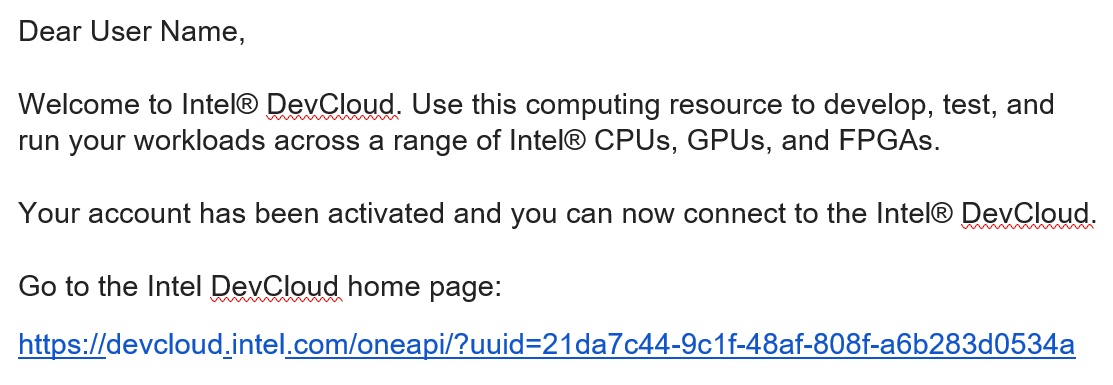
\includegraphics[scale=0.8]{figures/welcome.png}
   \caption{A part of the DevCloud welcome message.} 
	 \label{fig:welcome}
	 \end{center}
\end{figure}

\begin{figure}[H]
   \begin{center}
      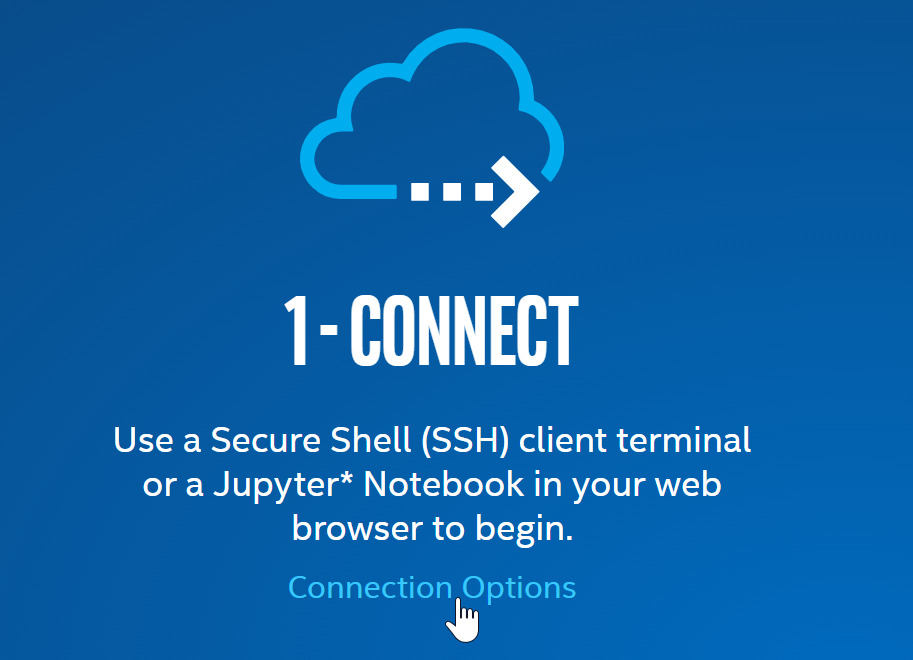
\includegraphics[scale=0.8]{figures/connect.png}
   \caption{Connect to the DevCloud.} 
	 \label{fig:connect}
	 \end{center}
\end{figure}

\begin{figure}[H]
   \begin{center}
      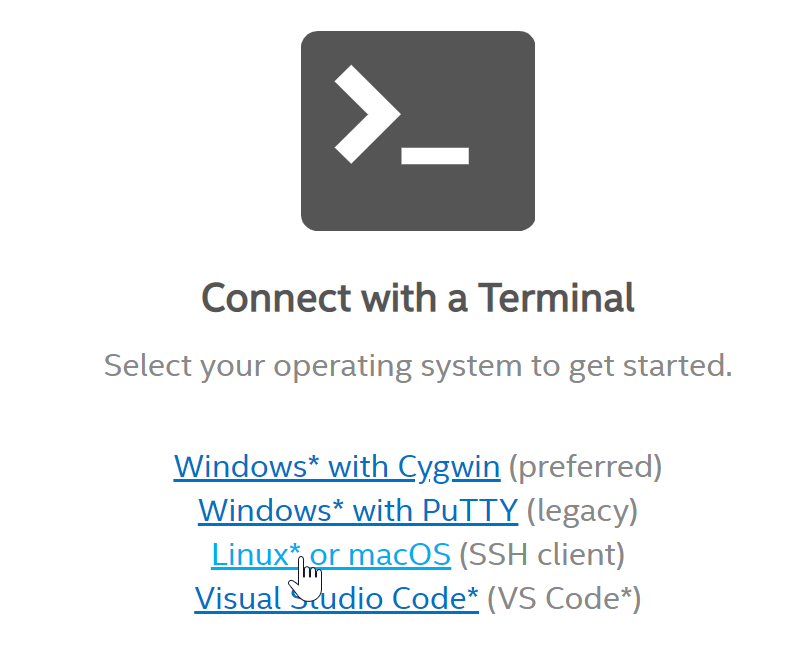
\includegraphics[scale=0.8]{figures/connect_terminal.png}
   \caption{Connection options.} 
	 \label{fig:connect_terminal}
	 \end{center}
\end{figure}

As indicated in Figure~\ref{fig:connect_terminal}, you should click to select the item 
labeled \blue{Linux$^*$ or macOS} {\sf (SSH client)}. This action opens a webpage customized to
your DevCloud login information, as illustrated in Figure~\ref{fig:ssh}. The DevCloud account
indicated in the figure, \texttt{u42132}, is shown for illustrative purposes only--the
webpage is customized to set up each user's unique DevCloud account.

\begin{figure}[H]
   \begin{center}
      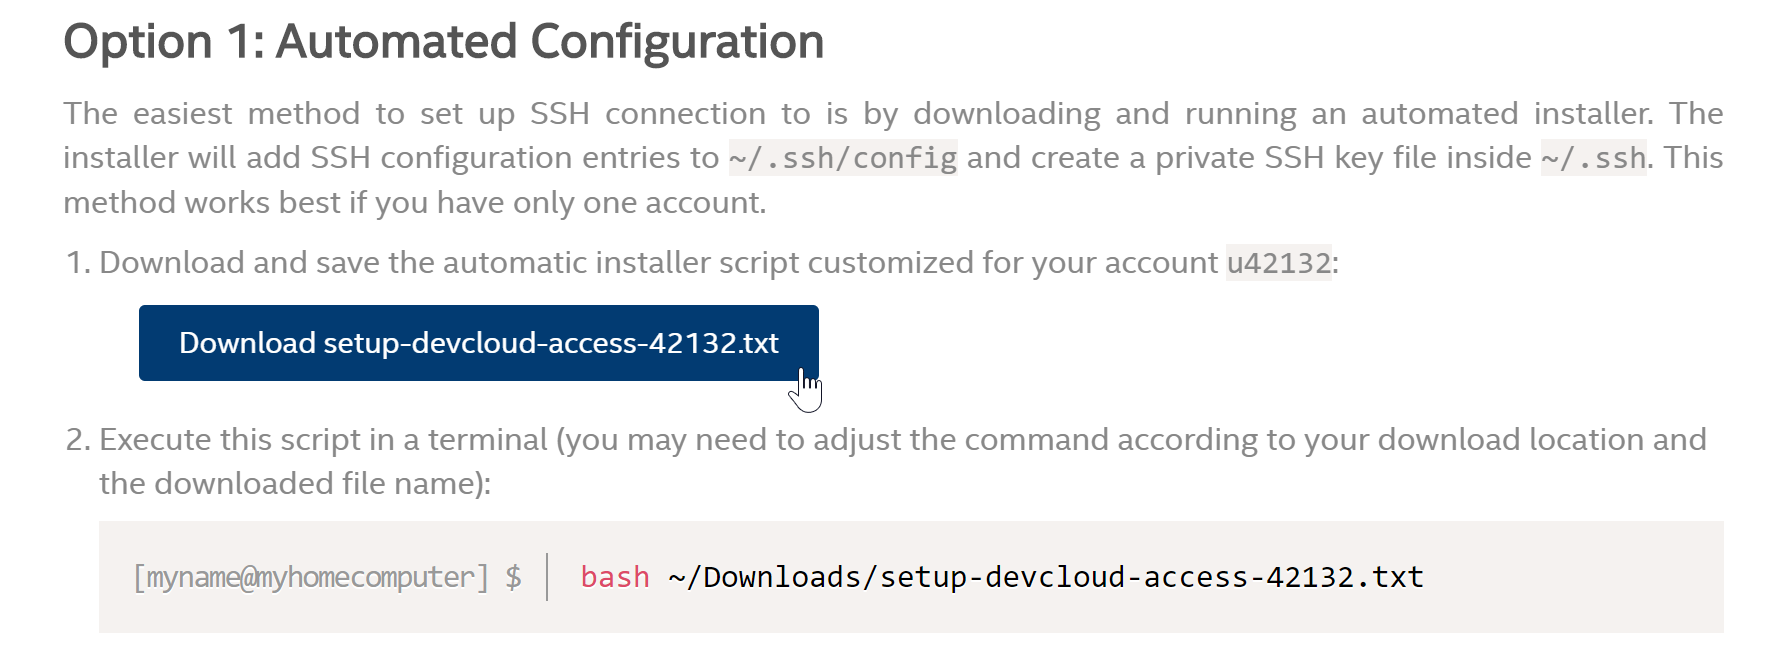
\includegraphics[width=\textwidth]{figures/ssh.png}
   \caption{Setting up a secure connection to the DevCloud.} 
	 \label{fig:ssh}
	 \end{center}
\end{figure}

By clicking on the dark-blue box in ``step \texttt{1}'' of Figure~\ref{fig:ssh} you can download a 
file onto your home computer that contains your DevCloud secure login information, 
in {\it Secure Shell} (SSH) format.
Before you can follow ``step \texttt{2}'' of Figure~\ref{fig:ssh} you have to be using a
Linux environment, as discussed below.

\subsection{Using Linux to Connect to the DevCloud} 
The SSH information downloaded using the link in Figure~\ref{fig:ssh} requires 
a Linux environment. If you are already using a Linux system, then you can skip
to Section~\ref{sec:ssh}. But if you are using Microsoft Windows, then a Linux environment 
has to be set up before continuing. We assume that
you are running Linux via the Microsoft Windows extension called 
{\it Windows System for Linux} (WSL). If you are using another method of accessing Linux, 
for example the {\it Cygwin} tools, then some differences may apply in the setup process.

If not already done on your computer, enable WSL. Instructions for enabling this feature of
Windows can be found by searching on the Internet. After WSL is enabled, download and
install the \texttt{Ubuntu} app from the Microsoft Windows Store. Open the Ubuntu app,
which provides you with a Linux terminal.

\subsubsection{Installing SSH Authentication} 
\label{sec:ssh}
To complete ``step \texttt{2}'' of Figure~\ref{fig:ssh}, in a Linux terminal execute the command 
\lstset{language=,numbers=none,escapechar=|}
\begin{lstlisting}
bash PATH/setup-devcloud-access-``userid''.txt
\end{lstlisting}

where \texttt{PATH} represents the directory where the ``setup'' file was saved when it was
downloaded in ``step 1''. This command extracts the SSH authentication information from the
setup file and stores it into your Linux user's home directory in $\sim$/.{\it ssh}. As 
a final step modify a file permission by executing the command
\begin{lstlisting}
chmod 600 ~/.ssh/config
\end{lstlisting}

Now, login to the DevCloud by executing the command
\begin{lstlisting}
ssh devcloud
\end{lstlisting}

Once logged in, perform the following one-time set up. Edit the .{\it bashrc} file
in your home directory on the DevCloud. Several {\it command-line interface} (CLI) text 
editors are available on the DevCloud, including {\it Vim}, {\it emacs}, {\it nano}, and 
{\it pico}. At the end of your 
.{\it bashrc} file append the line
\begin{lstlisting}
source /data/intel_fpga/devcloudLoginToolSetup.sh
\end{lstlisting}
This setting ensures that your environment is properly configured to execute additional
commands that are needed for AFU development.  To apply this new setting to your login session, 
logout of the DevCloud by typing either the end-of-transmission character 
$^\wedge$\texttt{D} (hold down the \texttt{CTRL} key and press \texttt{d}), 
or \texttt{exit}, and then login again by executing \texttt{ssh devcloud}.

\section{Using the DevCloud}
The command \texttt{ssh devcloud} makes a connection to a DevCloud computer named {\it login-2}. 
This machine does not have access to any FPGA accelerator cards. To connect to a computer
that has the required hardware resources execute (on {\it login-2}) the command
\begin{lstlisting}
devcloud_login
\end{lstlisting}

This command allows you to make a connection to machines that offer five different types of
compute-resources. For this tutorial we assume that AFU development will be done using 
an Arria 10 FPGA. If a different type of FPGA were to be used instead, then some of the 
instructions below would need to be modified accordingly.  Type \texttt{1} to select
\begin{lstlisting}
1) Arria 10 PAC Compilation and Programming - RTL AFU, OpenCL
\end{lstlisting}
You will then be presented with a choice of two versions of Arria 10 development tools. 
Type \texttt{1} to select
\begin{lstlisting}
1) 1.2.1
\end{lstlisting}

You should now be connected to a computer that includes an Arria 10 FPGA card. In this
discussion we assume that the computer is named {\it s005-n003}. To complete your setup, 
execute (on {\it s005-n003}) the command
\begin{lstlisting}
tools_setup
\end{lstlisting}

This command presents seven options for selecting development software. Type \texttt{5} to
choose
\begin{lstlisting}
5) Arria 10 PAC Compilation and Programming - RTL AFU, OpenCL
\end{lstlisting}

At this point the environment should be configured for access to the AFU development tools.
One of the software packages that we will use is called the 
{\it Open Programmable Accelerator Engine} (OPAE), which is part of the Intel Acceleration
Stack.  To verify the proper setup, type the command
\begin{lstlisting}
echo |\$|OPAE_PLATFORM_ROOT
\end{lstlisting}

This command should produce an output like the one illustrated in Figure~\ref{fig:setup}.
The OPAE software is installed on the DevCloud, and is also available in open-source form on
{\it GitHub} at \blue{https://github.com/OPAE}. This repository includes detailed documentation 
about OPAE.

~\\
\begin{figure}[H]
   \begin{center}
      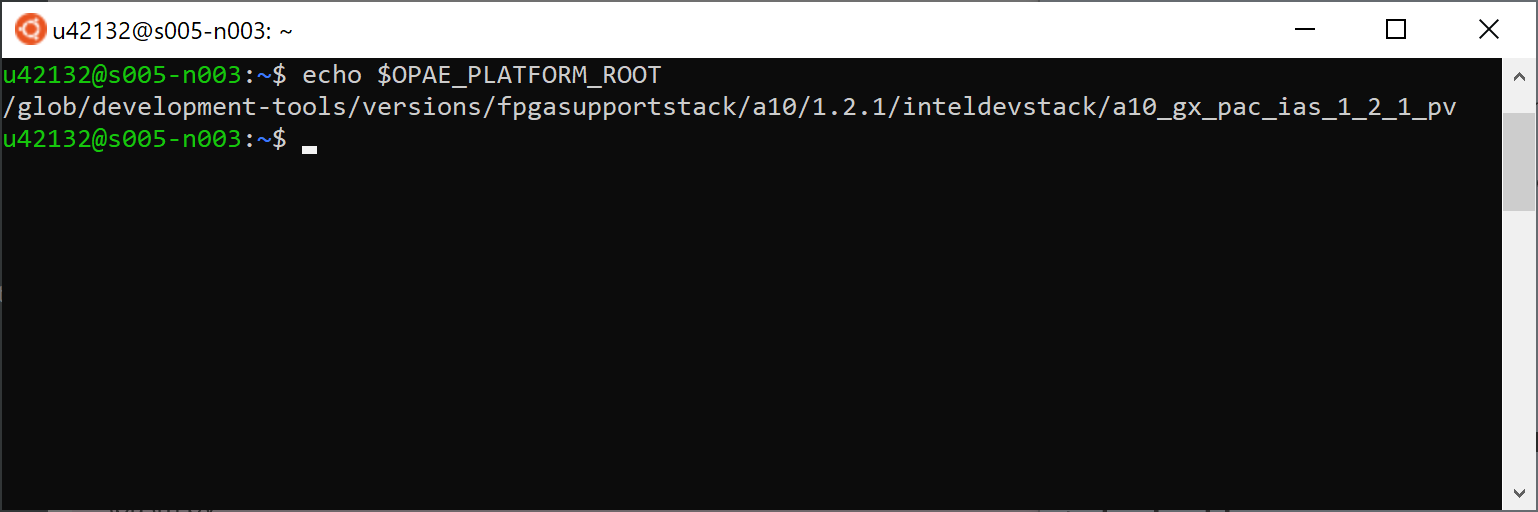
\includegraphics[width=\textwidth]{figures/setup.png}
   \caption{Verifying the proper setup.} 
	 \label{fig:setup}
	 \end{center}
\end{figure}

\subsection{Copying Files to/from the DevCloud}
Files that are created on your home computer can be copied onto the DevCloud. One simple
way to perform the desired file-transfer is to use the {\it Secure Copy} (\texttt{scp}) program. 
For example, to copy {\it homefile} from your computer to your
{\it home} directory ($\sim$) on the DevCloud you would use the command
\begin{lstlisting}
scp homefile devcloud:~/
\end{lstlisting}

Of course, you can copy files to other directories on the DevCloud by including the desired path
in the \texttt{scp} command. Similarly, \texttt{scp} can be used to copy a file from the 
DevCloud to the your home computer. For example, to copy {\it devfile} from the DevCloud to 
the current working directory (\texttt{.}) on your home computer you would use the command
\begin{lstlisting}
scp devcloud:~/devfile .
\end{lstlisting}

The \texttt{scp} command can by used to copy an entire directory {\it tree}, including 
sub-directories, by using the \texttt{-r} option. More information about \texttt{scp} can 
be found by typing \texttt{man scp}. Note that \texttt{scp} should be used with some
caution, as it {\it clobbers} (overwrites) existing files without warning. Thus, if you 
copy a file to a remote computer using \texttt{scp}, the file is overwritten on the remote 
computer if it already exists.

\subsection{Working with an AFU}
Intel documentation specifies that the source files for an AFU have to be structured in a
particular way. An example of a simple AFU, named {\it hello\_afu}, is provided as a sample 
on the DevCloud in the directory 
\begin{lstlisting}
|\$|OPAE_PLATFORM_ROOT/hw/samples
\end{lstlisting}
The AFU has a root directory called \texttt{hello\_afu}, which
contains directories named \texttt{hw} and \texttt{sw}. The \texttt{hw} directory contains a 
directory called \texttt{rtl}, which holds the hardware source-code files.
Figure~\ref{fig:sample} (near the top) shows the contents of the sample \texttt{rtl}
folder. With your working directory set to \texttt{samples}, copy \texttt{hello\_afu} to your home directory with the command \texttt{cp -r hello\_afu \textasciitilde}. If you create a new AFU, then before it can be compiled for the first time you must complete the following steps, using \texttt{hello\_afu} as an example. Run \texttt{cd \textasciitilde/hello\_afu} then execute the 
command
\begin{lstlisting}
afu_synth_setup --source hw/rtl/filelist.txt build_synth
\end{lstlisting}

\begin{figure}[H]
   \begin{center}
      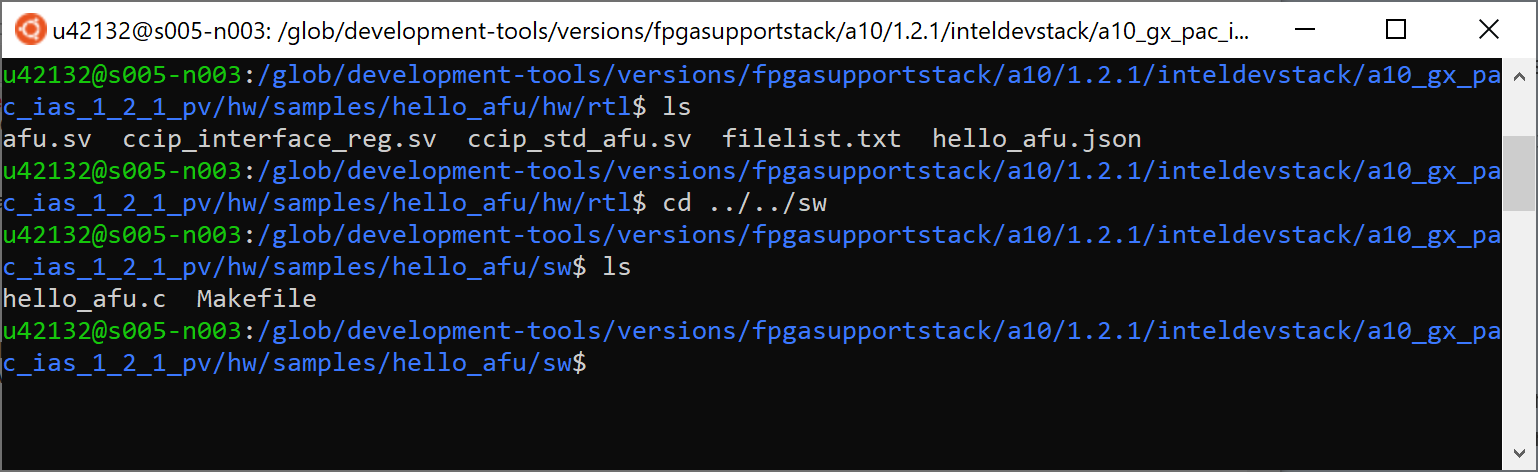
\includegraphics[scale=0.7]{figures/sample.png}
   \caption{Sample AFU hardware source-code files.} 
	 \label{fig:sample}
	 \end{center}
\end{figure}

This command creates the directory named \texttt{build\_synth} inside the \texttt{hello\_afu}
directory, and copies a number of files that are needed to compile the AFU into a hardware
circuit. To perform the hardware compilation you would set your working directory to 
\texttt{build\_synth} and execute the command
\begin{lstlisting}
run.sh
\end{lstlisting}

This command, which is found in the directory $\$$\texttt{OPAE\_PLATFORM\_ROOT/bin}, runs the
tools required to generate a hardware circuit for the AFU. In the case of the {\it hello\_afu}
example the circuit would be saved in a bitstream file called {\it hello\_afu.gbs}.

Some of the files created during hardware compilation can be ``cleaned up'' by executing
in the \texttt{build\_synth} directory the command
\begin{lstlisting}
clean.sh
\end{lstlisting}

\subsubsection{Downloading an AFU Bitstream into an FPGA}

You can download a bitstream file such as {\it hello\_afu.gbs} into an FPGA using a 
two-step process.  First, execute the command 
\begin{lstlisting}
PACSign PR -t UPDATE -H openssl_manager -i hello_afu.gbs -o hello_afu_unsigned.gbs
\end{lstlisting}

Then, execute
\begin{lstlisting}
fpgasupdate hello_afu_unsigned.gbs
\end{lstlisting}

\subsubsection{Compiling Software Programs for an AFU}
Software programs that utilize an AFU have to be contained in its \texttt{sw} directory.
These files can be compiled into executable programs by using a special {\it Makefile}. An
example Makefile, as well as a C source-code file, can be found in the \texttt{sw} folder 
for {\it hello\_afu}, as illustrated in Figure~\ref{fig:sample} (near the bottom).

\subsubsection{Miscellaneous Commands}
Some miscellaneous Linux and DevCloud <{\it commands}> are described below.

\begin{description}
\item [< ! >] You can use \texttt{!} to recall a previously executed command. 
For example, to
re-execute a previous \texttt{ssh} command you can type \texttt{!shh}. The Linux shell will 
search your command history for the last command that started with {\it ssh} and execute it again.
\item [< !:p >] This command is similar to \texttt{!,} except that is does not 
{\it execute} the
recalled command. For example, if you wish to check for the most-recently executed command
that begins with {\it ssh}, you would type \texttt{!ssh:p}.
\item [< $\uparrow$ >] You can use $\uparrow$ to recall previously-executed commands.
\item [< $^\wedge$Z >] When you are using a program, for example a text editor, typing 
$^\wedge$Z (hold down the \texttt{CTRL} key and press \texttt{z})
returns control to the Linux command-line prompt, but leaves your program
running in the {\it background}.
\item [< $\sim^\wedge$Z >] When you are connected to a {\it remote} computer, typing the
character sequence $\sim^\wedge$Z returns control to your {\it local} computer, but keeps the
session on the remote computer running in the {\it background}.
\item [< bg >] This command displays a list of all programs that you are running in 
the background.
\item [< fg >] The \texttt{fg} command returns control to the most recently-suspended 
background program. If there are multiple background programs then you can return control to 
program $n$ by executing \texttt{fg \%n}.
\item [< ps >] This command provides a list of currently-executing processes.
\item [< kill >] The \texttt{kill} command can be used to terminate a process.
\item [< killall >] Occasionally you may get automatically logged out of a compute-machine
on the DevCloud, for example the machine {\it s005-n003}, even though you have not purposely 
logged out. If this occurs then a subsequent issue may develop. Specifically, trying to reconnect
to a compute-machine using the command \texttt{devcloud\_login} may result in the error
\begin{lstlisting}
You are already logged into node =s005-n003 interactively.
\end{lstlisting}

In this case, you can reconnect to the machine by executing
\begin{lstlisting}
ssh s005-n003
\end{lstlisting}

After reconnecting, in some situations you may find that commands on the DevCloud do not
work properly. If this happens, then (as a last resort) you can kill all processes owned by 
your {\it userid}, by using the \texttt{killall} command. For example, if your userid 
were {\it u42132} you would type
\begin{lstlisting}
killall --user u42132
\end{lstlisting}

This command should terminate all processes owned by you and then disconnect from the
machine. If you do not get logged out, then execute the command one more time. 
\item [< uuidgen >] This DevCloud command generates a {\it universally unique identifier} (uuid) 
for an AFU.
\item [< pbsnodes >] This DevCloud command provides a listing of available compute-machines. To 
control the display of this list use the command \texttt{pbsnodes | more}.
\end{description}

\section{Concluding Remarks}

This tutorial has provided an introduction to the Intel FPGA DevCloud for AFU development.
Further details about the DevCloud can be found on its {\it GitHub} site 
at \blue{https://github.com/intel/FPGA-Devcloud}.

% Copyright and Trademark

%\newcommand{\datePublished}{Mar 2022}

\newcommand{\versnum}{21.1} %version number quartus/AMP
\newcommand{\quartusname}{Quartus\textsuperscript{\textregistered} Prime}	
\newcommand{\textBar}{For \quartusname{} \versnum{}}
\newcommand{\thisyear}{2022 } %for copyright
\newcommand{\company}{FPGAcademy.org}
\newcommand{\longteamname}{FPGAcademy.org}
\newcommand{\teamname}{FPGAcademy}
\newcommand{\website}{FPGAcademy.org}

\newcommand{\productAcronym}{AMP}
\newcommand{\productNameShort}{Monitor Program}

\newcommand{\productNameMedTM}{Monitor Program}
\newcommand{\productNameMed}{Monitor Program}

%\newcommand{\headerLogoFilePath}[1]{#1/FPGAcademy.png}



%%%%%%%%%%%%%%%%%%%%%%%%%%%%%%%%%%%%%%%%
%%% FPGAcademy Copyright Information %%%
%%%%%%%%%%%%%%%%%%%%%%%%%%%%%%%%%%%%%%%%

%Always put the copyright on a new page (clear page), with some vertical space from top
\clearpage
\vspace{1in}

\noindent

Copyright {\copyright} FPGAcademy.org. All rights reserved. FPGAcademy and the FPGAcademy logo are trademarks of  FPGAcademy.org.  This document is being provided on an ``as-is'' basis and as an accommodation and therefore all warranties, representations or guarantees of any kind (whether express, implied or statutory) including, without limitation, warranties of merchantability, non-infringement, or fitness for a particular purpose, are specifically disclaimed.

%FPGAcademy assumes no responsibility or liability arising out of the application or use of any information,  product,  or  service  described  herein  except  as  expressly  agreed  to  in  writing  by  FPGAcademy.



**Other names and brands may be claimed as the property of others.




\end{document}
